%!TEX root = thesis.tex

\chapter{Payment terminal acceptance testing}
\label{chapter:Payment terminal acceptance testing} 

When developing software with agile methodologies for payment terminals, i.e for embedded system, testing is a crucial part of the process. The earlier the defects and errors in the software are detected, the lower the cost and needed effort will be for correcting those (\emph{\cite{myers2011art}}).

Motivation for this research came from payment terminal software provider as they needed cost efficient and simple as possible automated acceptance test environment in order to lower the costs and speed up the acceptance testing phase of their software development.

In order to automate the acceptance testing of the payment terminals, test environment that can manipulate an observe the device through physical world has to be created. In other words, environment has to have some sort of a robot for pressing the buttons, screen of the device has to be observed and all this must be controlled by some kind of combination of software.

Test environment that can be used in acceptance testing of payment terminals has several challenges to tackle and matters related to physical and technical aspects of the payment terminals have to be considered. This chapter will discuss the background of these challenges. Customer also had desire for open source technologies and this chapter will discuss the benefits obtained by using open source software and and hardware in acceptance testing environment for payment terminals. Chapter will also discuss the different approaches for acceptance testing as well as how should the test suites be defined in order to make them understandable and reusable.

\section{Benefits of Open Source solutions}

\emph{\cite{paulson2004empirical}}



"Open source" hardware on the other hand means that details and plans of the product and parts are commonly available. This allows that parts can be manufactured and modified by anyone with knowledge and skills to suit individual needs. When detailed part descriptions are available multiple manufacturers can fabricate the parts. This creates competition and therefore usually lowers the price of individual hardware parts.

\section{Common characteristics between payment terminals}

When designing automated test environment for different kinds of payment terminals, different physical and technical features have to be taken into account. Environment has to be able to manipulate different types of payment terminals and test structure has to be designed to adapt to needs of different software and software versions running on payment terminals.

Almost all payment terminals share some common characteristics as they are made for same purpose: handling card payments. Scope of this thesis is to view those payment terminals that share three main features: keyboard, screen and card slot. Different types of terminals can be observed in Figure~\ref{fig:terminals} and Figure~\ref{fig:izettle} bellow.

Screens of the payment terminals differ in terms of size, placement and type. Test environment has to take into account different screen placements and it has to support both black and white (BW) and colored displays.

Keyboards of payment terminals share majority of keys together as number keys are needed for entering the PIN code and accept and decline buttons are needed for accepting and canceling the payment. Keyboard layouts, however, differ between different manufacturers and even amongst different models of the same manufacturer.

Location of the chip card slot is usually on the lover edge of the payment terminal or on top of the screen of the payment terminal. Research done within this thesis is limited to those terminals that have the chip card slot at the lower edge of the payment terminal as this simplifies the hardware needed for test environment. This is described more in depth in Chapter~\ref{section:Proposed hardware}. This study is also limited to only chip card readers and magnetic stripe readers or near field communication (NFC) payments are not addressed.





\begin{figure}[ht]
  \begin{center}
    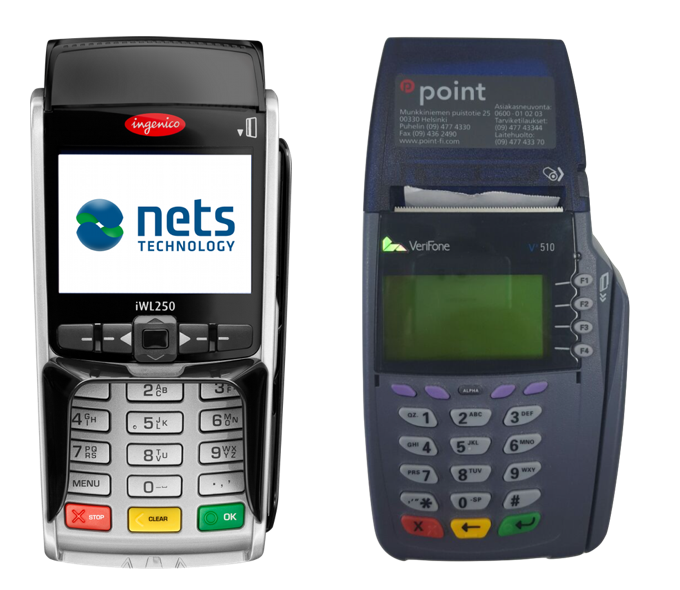
\includegraphics[width=9cm]{images/terminal1.png}
    \caption{Two examples of payment terminals from different manufacturers. Left image from: \url{http://www.netskauppa.fi/images/t/24-85-PrimaryImage.image.ashx}}
    \label{fig:terminals}
  \end{center}
\end{figure}

\begin{figure}[ht]
  \begin{center}
    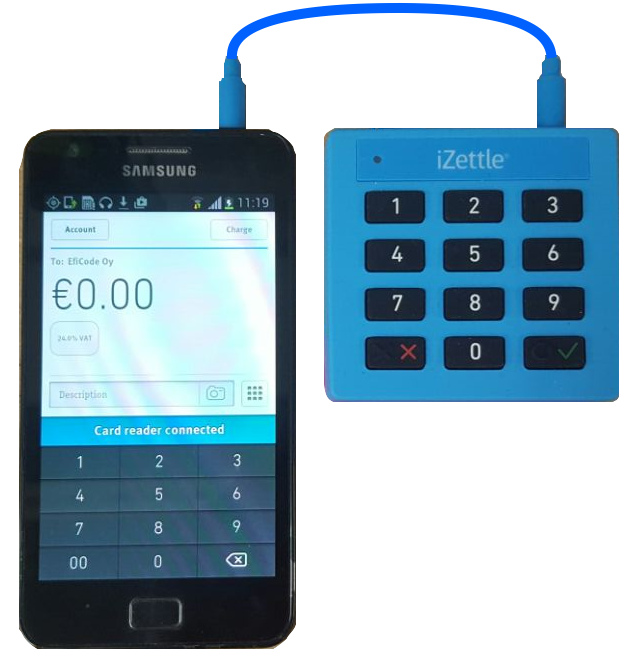
\includegraphics[width=8cm]{images/izettle.png}
    \caption{Example of a payment terminal which attaches to a smart phone.}
    \label{fig:izettle}
  \end{center}
\end{figure}

\section{Different approaches for test automation}

\emph{\cite{khan2012comparative}}


\section{Test suite syntax}


\begin{figure}[ht]
  \begin{center}
    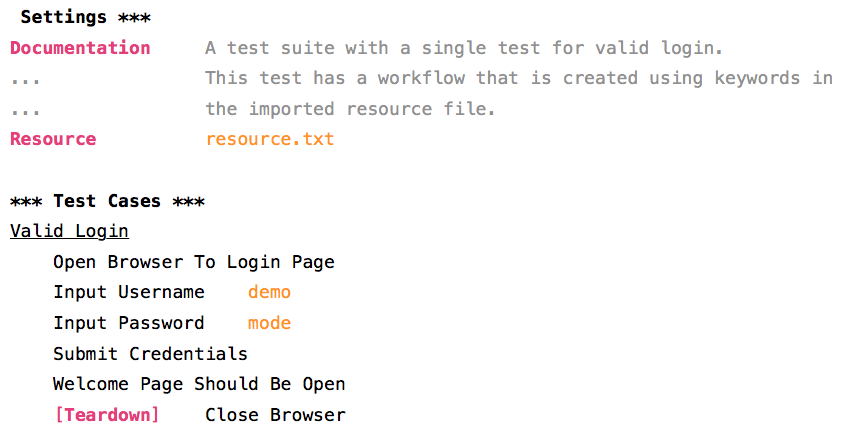
\includegraphics[width=10cm]{images/robot_example.png}
    \caption{Example of a simple test suite. Source: \url{http://robotframework.org}}
    \label{fig:robot_example}
  \end{center}
\end{figure}
